\documentclass[11pt,]{problemset}
\usepackage{lmodern}
\usepackage{amssymb,amsmath}
\usepackage{ifxetex,ifluatex}
\usepackage{fixltx2e} % provides \textsubscript
\ifnum 0\ifxetex 1\fi\ifluatex 1\fi=0 % if pdftex
  \usepackage[T1]{fontenc}
  \usepackage[utf8]{inputenc}
\else % if luatex or xelatex
  \ifxetex
    \usepackage{mathspec}
  \else
    \usepackage{fontspec}
  \fi
  \defaultfontfeatures{Ligatures=TeX,Scale=MatchLowercase}
    \setmainfont[]{IPAPMincho}
    \setsansfont[]{IPAPGothic}
\fi
% use upquote if available, for straight quotes in verbatim environments
\IfFileExists{upquote.sty}{\usepackage{upquote}}{}
% use microtype if available
\IfFileExists{microtype.sty}{%
\usepackage{microtype}
\UseMicrotypeSet[protrusion]{basicmath} % disable protrusion for tt fonts
}{}
\usepackage{hyperref}
\hypersetup{unicode=true,
            pdfborder={0 0 0},
            breaklinks=true}
\urlstyle{same}  % don't use monospace font for urls
\usepackage{color}
\usepackage{fancyvrb}
\newcommand{\VerbBar}{|}
\newcommand{\VERB}{\Verb[commandchars=\\\{\}]}
\DefineVerbatimEnvironment{Highlighting}{Verbatim}{commandchars=\\\{\}}
% Add ',fontsize=\small' for more characters per line
\usepackage{framed}
\definecolor{shadecolor}{RGB}{248,248,248}
\newenvironment{Shaded}{\begin{snugshade}}{\end{snugshade}}
\newcommand{\AlertTok}[1]{\textcolor[rgb]{0.94,0.16,0.16}{#1}}
\newcommand{\AnnotationTok}[1]{\textcolor[rgb]{0.56,0.35,0.01}{\textbf{\textit{#1}}}}
\newcommand{\AttributeTok}[1]{\textcolor[rgb]{0.77,0.63,0.00}{#1}}
\newcommand{\BaseNTok}[1]{\textcolor[rgb]{0.00,0.00,0.81}{#1}}
\newcommand{\BuiltInTok}[1]{#1}
\newcommand{\CharTok}[1]{\textcolor[rgb]{0.31,0.60,0.02}{#1}}
\newcommand{\CommentTok}[1]{\textcolor[rgb]{0.56,0.35,0.01}{\textit{#1}}}
\newcommand{\CommentVarTok}[1]{\textcolor[rgb]{0.56,0.35,0.01}{\textbf{\textit{#1}}}}
\newcommand{\ConstantTok}[1]{\textcolor[rgb]{0.00,0.00,0.00}{#1}}
\newcommand{\ControlFlowTok}[1]{\textcolor[rgb]{0.13,0.29,0.53}{\textbf{#1}}}
\newcommand{\DataTypeTok}[1]{\textcolor[rgb]{0.13,0.29,0.53}{#1}}
\newcommand{\DecValTok}[1]{\textcolor[rgb]{0.00,0.00,0.81}{#1}}
\newcommand{\DocumentationTok}[1]{\textcolor[rgb]{0.56,0.35,0.01}{\textbf{\textit{#1}}}}
\newcommand{\ErrorTok}[1]{\textcolor[rgb]{0.64,0.00,0.00}{\textbf{#1}}}
\newcommand{\ExtensionTok}[1]{#1}
\newcommand{\FloatTok}[1]{\textcolor[rgb]{0.00,0.00,0.81}{#1}}
\newcommand{\FunctionTok}[1]{\textcolor[rgb]{0.00,0.00,0.00}{#1}}
\newcommand{\ImportTok}[1]{#1}
\newcommand{\InformationTok}[1]{\textcolor[rgb]{0.56,0.35,0.01}{\textbf{\textit{#1}}}}
\newcommand{\KeywordTok}[1]{\textcolor[rgb]{0.13,0.29,0.53}{\textbf{#1}}}
\newcommand{\NormalTok}[1]{#1}
\newcommand{\OperatorTok}[1]{\textcolor[rgb]{0.81,0.36,0.00}{\textbf{#1}}}
\newcommand{\OtherTok}[1]{\textcolor[rgb]{0.56,0.35,0.01}{#1}}
\newcommand{\PreprocessorTok}[1]{\textcolor[rgb]{0.56,0.35,0.01}{\textit{#1}}}
\newcommand{\RegionMarkerTok}[1]{#1}
\newcommand{\SpecialCharTok}[1]{\textcolor[rgb]{0.00,0.00,0.00}{#1}}
\newcommand{\SpecialStringTok}[1]{\textcolor[rgb]{0.31,0.60,0.02}{#1}}
\newcommand{\StringTok}[1]{\textcolor[rgb]{0.31,0.60,0.02}{#1}}
\newcommand{\VariableTok}[1]{\textcolor[rgb]{0.00,0.00,0.00}{#1}}
\newcommand{\VerbatimStringTok}[1]{\textcolor[rgb]{0.31,0.60,0.02}{#1}}
\newcommand{\WarningTok}[1]{\textcolor[rgb]{0.56,0.35,0.01}{\textbf{\textit{#1}}}}
\usepackage{graphicx,grffile}
\makeatletter
\def\maxwidth{\ifdim\Gin@nat@width>\linewidth\linewidth\else\Gin@nat@width\fi}
\def\maxheight{\ifdim\Gin@nat@height>\textheight\textheight\else\Gin@nat@height\fi}
\makeatother
% Scale images if necessary, so that they will not overflow the page
% margins by default, and it is still possible to overwrite the defaults
% using explicit options in \includegraphics[width, height, ...]{}
\setkeys{Gin}{width=\maxwidth,height=\maxheight,keepaspectratio}
\IfFileExists{parskip.sty}{%
\usepackage{parskip}
}{% else
\setlength{\parindent}{0pt}
\setlength{\parskip}{6pt plus 2pt minus 1pt}
}
\setlength{\emergencystretch}{3em}  % prevent overfull lines
\providecommand{\tightlist}{%
  \setlength{\itemsep}{0pt}\setlength{\parskip}{0pt}}
\setcounter{secnumdepth}{0}
% Redefines (sub)paragraphs to behave more like sections
\ifx\paragraph\undefined\else
\let\oldparagraph\paragraph
\renewcommand{\paragraph}[1]{\oldparagraph{#1}\mbox{}}
\fi
\ifx\subparagraph\undefined\else
\let\oldsubparagraph\subparagraph
\renewcommand{\subparagraph}[1]{\oldsubparagraph{#1}\mbox{}}
\fi

%%% Use protect on footnotes to avoid problems with footnotes in titles
\let\rmarkdownfootnote\footnote%
\def\footnote{\protect\rmarkdownfootnote}

%%% Change title format to be more compact
\usepackage{titling}

% Create subtitle command for use in maketitle
\providecommand{\subtitle}[1]{
  \posttitle{
    \begin{center}\large#1\end{center}
    }
}

\setlength{\droptitle}{-2em}

  \title{}
    \pretitle{\vspace{\droptitle}}
  \posttitle{}
    \author{}
    \preauthor{}\postauthor{}
    \date{}
    \predate{}\postdate{}
  
\usepackage{sectsty}
\usepackage{tikz}
\usetikzlibrary{trees}
\usepackage{mathspec}
\usepackage{amsmath,amsthm}
\usepackage{amssymb,amsfonts}
\usepackage[all,arc]{xy}
\usepackage{enumerate}
\usepackage{mathrsfs}
\usepackage[margin=1in]{geometry}
\usepackage{thmtools}
\usepackage{verbatim}
\usepackage{xltxtra}
\XeTeXlinebreaklocale ``ja''
\XeTeXlinebreakskip=0pt plus 1pt
\XeTeXlinebreakpenalty=0
\setmainfont[]{IPAPMincho}
\setsansfont[]{IPAPGothic}
\usepackage{afterpage}
\sectionfont{\fontsize{12}{15}\selectfont}
\author{学籍番号:}
\course{疫学演習 2019-6-5 \& 2019-6-12}
\problemset{ }
\problem{ }
\collab{氏名:}

\begin{document}

\section{問題1:両群間計量データの平均値を比較する}

200名の認知症患者を募集し,認識能力テスト(cognitive test,
COG),及び脳萎縮の進行度 (brain atrophy,
脳体積の平均年間減少率,単位は\%)
の検査を全員に行った.COG,及び脳萎縮のデータは大きいほど認知症の進行度がより進んでいる.また,この200名の参加者から採取した血液検体を利用して,ある遺伝子の変異の有無を検査した.このデータは以下の表でまとめた:

\bigskip
\begin{center}
\begin{tabular}{|l|l|l|l|l|}\hline
変数                     & \multicolumn{2}{c|}{遺伝変異あり (n = 50)}     & \multicolumn{2}{c|}{遺伝変異なし (n = 150)}   \\\hline
                       & \vtop{\hbox{\strut 平均値}\hbox{\strut (mean)}}&\vtop{\hbox{\strut  標準偏差}\hbox{\strut (standard deviation) }} & \vtop{\hbox{\strut 平均値}\hbox{\strut (mean)}}&\vtop{\hbox{\strut  標準偏差}\hbox{\strut (standard deviation) }} \\\hline
認識能力テスト,COG            & 69.2       & 9.0                       & 60.2       & 9.0                       \\
脳萎縮度, atrophy, \%/year & 0.67       & 0.21                      & 0.23       & 0.10                     \\\hline
\end{tabular}
\end{center}
\bigskip

\begin{enumerate}
\def\labelenumi{\arabic{enumi}.}
\tightlist
\item
  帰無仮説を「遺伝子変異ありと変異なし両群の間に,COGの平均値は等しい」とする.上記のデータ及び適宜な方法を使って検定せよ.検定の結果を分かりやすく説明せよ.なお,分散が等しいと仮定できる場合,以下の式で両群の共通標準偏差が計算できる:
\end{enumerate}

\begin{equation}
  \label{eq:1}
S = \sqrt{\frac{(n_A - 1)S^2_A + (n_B - 1)S^2_B}{n_A + n_B -2}}
\end{equation}

\begin{itemize}
\tightlist
\item
  \(S_A:\) A群の標準偏差;
\item
  \(n_A:\) A群の人数;
\item
  \(S_B:\) B群の標準偏差;
\item
  \(n_B:\) B群の人数;
\item
  \(S:\) A群及びB群の共通標準偏差;
\item
  \(n_A + n_B -2:\) 分散が等しい時の自由度.
\end{itemize}

また,EZR で t 値,自由度 (degree of freedom)を使って P
値を計算する時,以下のコマンドを利用してください:

\begin{Shaded}
\begin{Highlighting}[]
\DecValTok{2}\OperatorTok{*}\KeywordTok{pt}\NormalTok{(t value, degree of freedom, }\DataTypeTok{lower=}\OtherTok{FALSE}\NormalTok{)}
\end{Highlighting}
\end{Shaded}

\newpage
\vfill

\subsection{答え}

両群の標準偏差は 9.0 と推定され,分散が等しいと仮定できるから,Student
の t 検定を行う:

\[
T = \frac{\bar{X}_A - \bar{X}_B}{S\sqrt{1/n_A + 1/n_B}}
\]

公式(\ref{eq:1})により,共通分散/標準偏差を推定する: \[
\begin{aligned}
\because\;\;  S & = \sqrt{\frac{(n_A - 1)S^2_A + (n_B - 1)S^2_B}{n_A + n_B -2}} \\
\therefore\;\; S & =  \sqrt{\frac{(50 - 1)9^2 + (150 - 1)9^2}{50 + 150 -2}} = 9 \\
\Rightarrow\;\; T & = \frac{\bar{X}_A - \bar{X}_B}{S\sqrt{1/n_A + 1/n_B}} \\ 
                  & = \frac{69.2 - 60.2}{9\times\sqrt{1/50 + 1/150}} \\ 
                  & = \frac{9}{9\times0.1633} = 6.1237
\end{aligned}
\]

自由度 (degree of freedom)は \(n_A + n_B -2 = 198\),P値の計算は EZR
を利用する:

\begin{Shaded}
\begin{Highlighting}[]
\DecValTok{2}\OperatorTok{*}\KeywordTok{pt}\NormalTok{(}\FloatTok{6.1237}\NormalTok{, }\DecValTok{198}\NormalTok{, }\DataTypeTok{lower=}\OtherTok{FALSE}\NormalTok{)}
\end{Highlighting}
\end{Shaded}

\begin{verbatim}
## [1] 4.831141e-09
\end{verbatim}

\begin{center}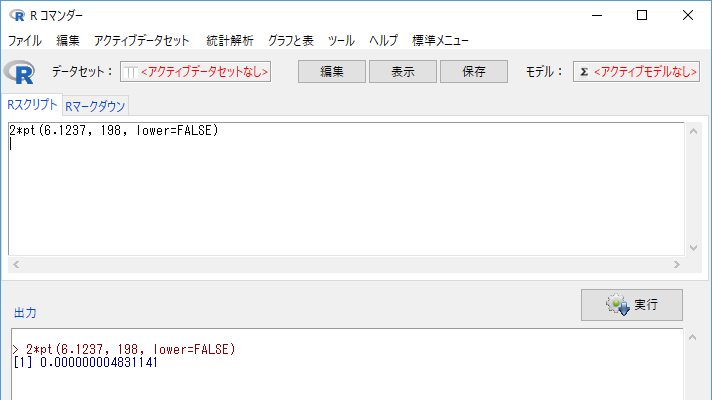
\includegraphics[width=0.9\linewidth]{pic/tvaluepvalue00} \end{center}
\bigskip

\newpage
\vfill

以下のコードをRスクリプトに入力して,実行をクリックしてください.自分の検定結果とは一致するかを確認してください.

\begin{Shaded}
\begin{Highlighting}[]
\KeywordTok{source}\NormalTok{(}\StringTok{"http://aoki2.si.gunma-u.ac.jp/R/src/my_t_test.R"}\NormalTok{, }\DataTypeTok{encoding=}\StringTok{"euc-jp"}\NormalTok{)}
\KeywordTok{my.t.test}\NormalTok{(}\DecValTok{50}\NormalTok{, }\FloatTok{69.2}\NormalTok{, }\FloatTok{9.0}\OperatorTok{^}\DecValTok{2}\NormalTok{, }\DecValTok{150}\NormalTok{, }\FloatTok{60.2}\NormalTok{, }\FloatTok{9.0}\OperatorTok{^}\DecValTok{2}\NormalTok{, }\DataTypeTok{var.equal=}\OtherTok{TRUE}\NormalTok{)}
\end{Highlighting}
\end{Shaded}

\begin{verbatim}
## 
##  等分散を仮定した,二群の平均値の差の検定
## 
## data:  
## n1 = 50, mean1 = 69.2, variance1 = 81
## n2 = 150, mean2 = 60.2, variance2 = 81
## t = 6.1237, df = 198, p-value = 4.831e-09
\end{verbatim}

\begin{center}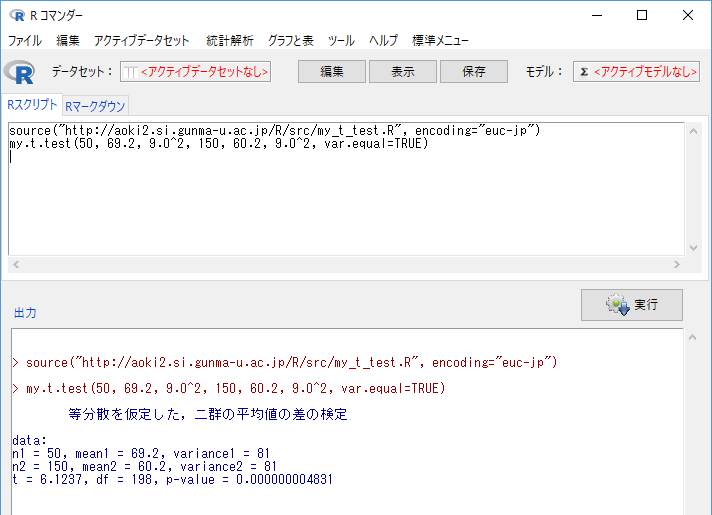
\includegraphics[width=0.9\linewidth]{pic/myttest01} \end{center}
\bigskip

\underline{手計算の結果とは一致していると確認できる.}

この検定結果は「両群のCOG平均値が等しい」という帰無仮説を棄却するために非常に強い証拠を提供したと言える.

There is strong evidence against the null hypothesis that the means of
COG are the same in the two groups.

\newpage
\vfill

\begin{enumerate}
\def\labelenumi{\arabic{enumi}.}
\setcounter{enumi}{1}
\tightlist
\item
  この患者データから,遺伝子変異ありとなしの群の間に脳萎縮度 (atrophy)
  の比較を 1. と同じ方法で検定してもよいか?どの検定方法を使えば 1.
  と同じ検定方法を使えるかどうかを判断できるを説明せよ.実際にこの検定方法を行ってください.
\end{enumerate}

なお,EZR で F 値,両群の分散,両群それぞれの自由度 (df) を使って P
値を計算する時に,以下のコマンドを利用してください:

\begin{Shaded}
\begin{Highlighting}[]
\DecValTok{2}\OperatorTok{*}\KeywordTok{pf}\NormalTok{(F value, df }\ControlFlowTok{in}\NormalTok{ group }\DecValTok{1}\NormalTok{, df }\ControlFlowTok{in}\NormalTok{ group }\DecValTok{2}\NormalTok{, }\DataTypeTok{lower=}\OtherTok{FALSE}\NormalTok{)}
\end{Highlighting}
\end{Shaded}

\hypertarget{-1}{%
\subsection{答え}\label{-1}}

テーブルから両群の標準偏差はそれぞれ 0.21, 0.10 だと推定され,分散
(variance)
が等しいという前提が満たされていない.1.の検定方法を使う時には,両群の分散が等しいという前提条件が必須だから,同じ
Student t
検定を行うことができない.「両群の分散」が等しいという帰無仮説を検定するには
F 検定を利用する:

\[
\begin{aligned}
F & = \frac{S^2_A}{S^2_B} \\
  & = \frac{0.21^2}{0.10^2} \\
  & = 4.41
\end{aligned}
\]

自由度 (degree of freedom)はそれぞれ
\(n_A - 1 = 49; n_B -2 = 149\),P値の計算は EZR を利用する:

\begin{Shaded}
\begin{Highlighting}[]
\DecValTok{2}\OperatorTok{*}\KeywordTok{pf}\NormalTok{(}\FloatTok{4.41}\NormalTok{, }\DecValTok{49}\NormalTok{, }\DecValTok{149}\NormalTok{, }\DataTypeTok{lower.tail =} \OtherTok{FALSE}\NormalTok{)}
\end{Highlighting}
\end{Shaded}

\begin{verbatim}
## [1] 2.971758e-12
\end{verbatim}

\begin{center}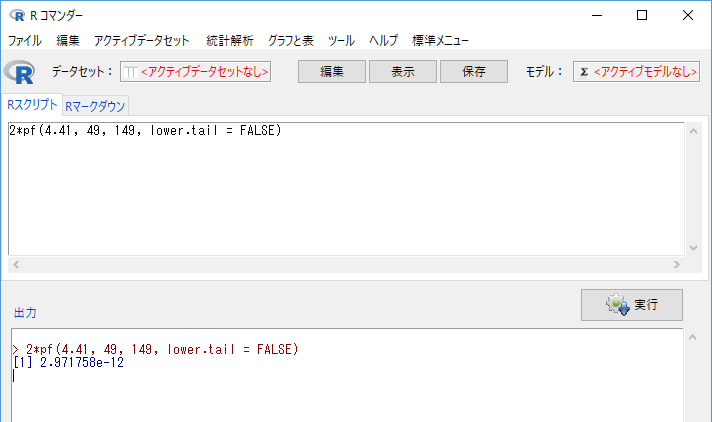
\includegraphics[width=0.9\linewidth]{pic/ftest} \end{center}
\bigskip

以下のコードをRスクリプトに入力して,実行をクリックしてください.自分の検定結果とは一致するかを確認してください.

\begin{Shaded}
\begin{Highlighting}[]
\KeywordTok{source}\NormalTok{(}\StringTok{"http://aoki2.si.gunma-u.ac.jp/R/src/my_var_test.R"}\NormalTok{, }\DataTypeTok{encoding=}\StringTok{"euc-jp"}\NormalTok{)}
\KeywordTok{my.var.test}\NormalTok{(}\DecValTok{50}\NormalTok{, }\FloatTok{0.21}\OperatorTok{^}\DecValTok{2}\NormalTok{, }\DecValTok{150}\NormalTok{, }\FloatTok{0.1}\OperatorTok{^}\DecValTok{2}\NormalTok{)}
\end{Highlighting}
\end{Shaded}

\begin{verbatim}
## 
##  二次データから,二群の等分散性の検定
## 
## data:  n1 = 50, variance1 = 0.0441, n2 = 150, variance2 = 0.01
## F = 4.41, num df = 49, denom df = 149, p-value = 2.972e-12
\end{verbatim}

\begin{center}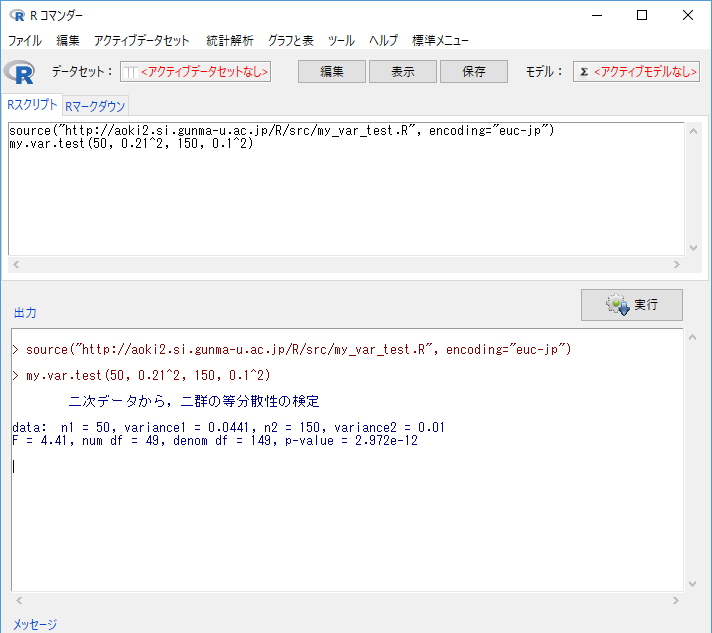
\includegraphics[width=0.9\linewidth]{pic/ftest01} \end{center}
\bigskip

\underline{手計算の結果とは一致していると確認できる.}

この検定結果は「両群の脳萎縮度の分散が等しい」という帰無仮説を棄却するために非常に強い証拠を提供したと言える.

There is strong evidence against the null hypothesis that the variances
of atrophy are the same in the two groups.

\newpage
\vfill

\begin{enumerate}
\def\labelenumi{\arabic{enumi}.}
\setcounter{enumi}{2}
\tightlist
\item
  2.の結果を踏まえて,帰無仮設「両群の脳萎縮度の平均値が等しい」を検定せよ.なお,両群の分散が等しいという前提が満たされていない時に,自由度(df)の計算式は以下となる:
\end{enumerate}

\begin{equation}
\label{eq:2}
\mathbf{df} = \frac{(S^2_A/n_A + S^2_B/n_B)^2}{(S_A^2/n_A)^2/(n_A-1)+(S_B^2/n_B)^2/(n_B-1)}
\end{equation}

また,EZR で t 値,自由度 (df)を使って P
値を計算する時,以下のコマンドを利用してください:

\begin{Shaded}
\begin{Highlighting}[]
\DecValTok{2}\OperatorTok{*}\KeywordTok{pt}\NormalTok{(t value, df, }\DataTypeTok{lower=}\OtherTok{FALSE}\NormalTok{)}
\end{Highlighting}
\end{Shaded}

\hypertarget{-2}{%
\subsection{答え}\label{-2}}

2.の検定結果から,「両群の脳萎縮度の分散が等しい」という帰無仮説を棄却されたため,Welch
の t 検定を採用する.

\[
\begin{aligned}
\Rightarrow\;\; T & = \frac{\bar{X}_A - \bar{X}_B}{\sqrt{S^2_A/n_A + S^2_B/n_B}} \\ 
                  & = \frac{0.67 - 0.23}{\sqrt{0.21^2/50 + 0.10^2/150}} \\ 
                  & = \frac{0.44}{\sqrt{0.0009486667}} = 14.28551
\end{aligned}
\]

自由度は公式(\ref{eq:2})により計算できる:

\[
\begin{aligned}
\mathbf{df} & = \frac{(S^2_A/n_A + S^2_B/n_B)^2}{(S_A^2/n_A)^2/(n_A-1)+(S_B^2/n_B)^2/(n_B-1)} \\
            & = \frac{(0.21^2/50 + 0.10^2/150)^2}{(0.21^2/50)^2/(50-1)+(0.10^2/150)^2/(150-1)} \\
            & = 58.58105
\end{aligned}
\] P値の計算は EZR を利用する:

\begin{Shaded}
\begin{Highlighting}[]
\DecValTok{2}\OperatorTok{*}\KeywordTok{pt}\NormalTok{(}\FloatTok{14.28551}\NormalTok{, }\FloatTok{58.58105}\NormalTok{, }\DataTypeTok{lower=}\OtherTok{FALSE}\NormalTok{)}
\end{Highlighting}
\end{Shaded}

\begin{verbatim}
## [1] 9.601543e-21
\end{verbatim}

\begin{center}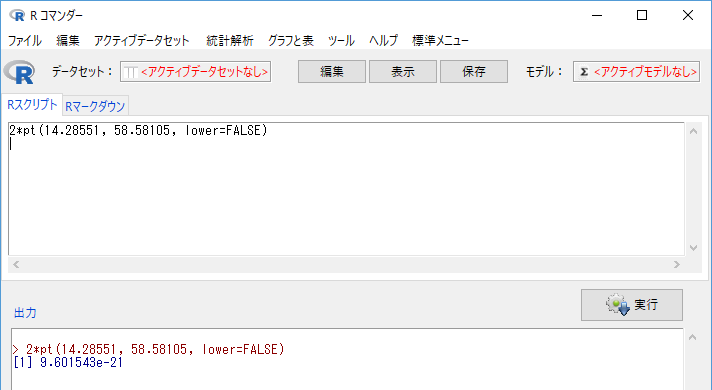
\includegraphics[width=0.9\linewidth]{pic/tvaluepvalue01} \end{center}
\bigskip

以下のコードをRスクリプトに入力して,実行をクリックしてください.自分の検定結果とは一致するかを確認してください.

\begin{Shaded}
\begin{Highlighting}[]
\KeywordTok{source}\NormalTok{(}\StringTok{"http://aoki2.si.gunma-u.ac.jp/R/src/my_t_test.R"}\NormalTok{, }\DataTypeTok{encoding=}\StringTok{"euc-jp"}\NormalTok{)}
\KeywordTok{my.t.test}\NormalTok{(}\DecValTok{50}\NormalTok{, }\FloatTok{0.67}\NormalTok{, }\FloatTok{0.21}\OperatorTok{^}\DecValTok{2}\NormalTok{, }\DecValTok{150}\NormalTok{, }\FloatTok{0.23}\NormalTok{, }\FloatTok{0.10}\OperatorTok{^}\DecValTok{2}\NormalTok{, }\DataTypeTok{var.equal=}\OtherTok{FALSE}\NormalTok{)}
\end{Highlighting}
\end{Shaded}

\begin{verbatim}
## 
##  ウエルチの方法による,二群の平均値の差の検定
## 
## data:  
## n1 = 50, mean1 = 0.67, variance1 = 0.0441
## n2 = 150, mean2 = 0.23, variance2 = 0.01
## t = 14.286, df = 56.581, p-value < 2.2e-16
\end{verbatim}

\begin{center}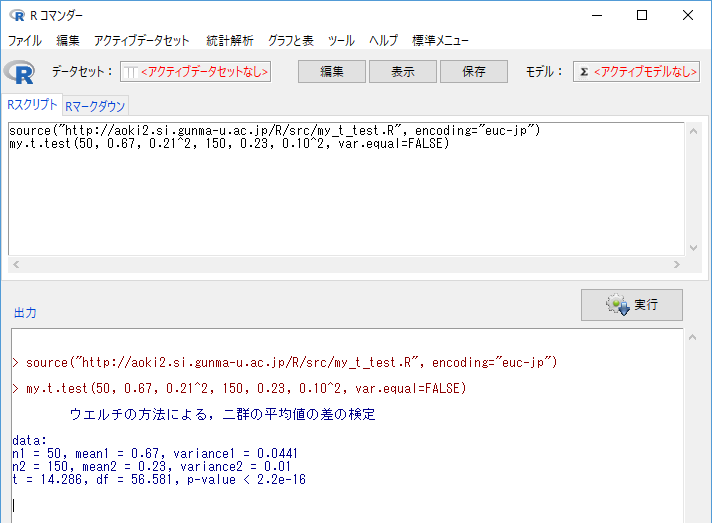
\includegraphics[width=0.9\linewidth]{pic/myttest02} \end{center}
\bigskip

\underline{手計算の結果とは一致していると確認できる.}

この検定結果は「両群の脳萎縮度の平均値が等しい」という帰無仮説を棄却するために非常に強い証拠を提供したと言える.

There is strong evidence against the null hypothesis that the means of
atrophy are the same in the two groups.

\newpage
\vfill

\section{問題2}

\newpage
\vfill

\section{参考図書:}

1.「Rによる保健医療データ解析演習」,中澤 港,(\url{http://minato.sip21c.org/msb/medstatbookx.pdf})
2.「みんなの医療統計 12日間で基礎理論とEZRを完全マスター!」,新谷 歩.


\end{document}
